% Submission: 4th eBPF Workshop (eBPF'26), co-located with ACM SOSP 2026
% Submission deadline: 2026-06-19
% Format: Research paper, 6 pages body + unlimited references
% Anonymity: double-blind for review submission

% \documentclass[sigconf,review,anonymous]{acmart}
\documentclass[sigplan,10pt]{acmart}
\settopmatter{printfolios=false}
\pagestyle{plain}

% --- ACM metadata (camera-ready; from the eRights confirmation) ---
\acmYear{2026}\copyrightyear{2026}
\setcopyright{cc}
\setcctype[4.0]{by}
\acmConference[eBPF '26]{4th Workshop on eBPF and Kernel Extensions}{September 29--October 2, 2026}{Prague, Czech Republic}
\acmBooktitle{4th Workshop on eBPF and Kernel Extensions (eBPF '26), September 29--October 2, 2026, Prague, Czech Republic}
\acmDOI{10.1145/3837779.3838166}
\acmISBN{979-8-4007-2911-9/26/09}

% \setcopyright{none}
% \acmConference[eBPF'26]{4th ACM SIGCOMM Workshop on eBPF and Kernel Extensions}{September 29, 2026}{Prague, Czech Republic}
% \acmYear{2026}
\settopmatter{printacmref=true, printccs=true, printfolios=false}

\citestyle{acmnumeric}

% Keep the running-header-to-text span within the 229mm the format
% checker measures: sigplan derives textheight from the fixed 1in
% top/bottom margins, so a larger bottom margin (51 lines, 622pt) is
% the knob. Body still ends on page 7.
\geometry{bottom=99pt}

% --- Packages ---
\usepackage{booktabs}
\usepackage{listings}
\usepackage{xcolor}
\usepackage{pifont}
\usepackage{xspace}
\usepackage{graphicx}
\usepackage[noend]{algpseudocode}
\usepackage{algorithm}

% --- Scoreboard marks for Table 4 (expressiveness) ---
% Use \partsym (not \partial) — \partial is the LaTeX kernel math symbol.
\newcommand{\yes}{\textcolor{green!55!black}{\ding{51}}}        % supported
\newcommand{\no}{\textcolor{red!70!black}{\ding{55}}}            % unsupported
\newcommand{\partsym}{\textcolor{orange!85!black}{$\sim$}}       % partial / awkward
\newcommand{\na}{\textcolor{gray}{\textemdash}}                  % not applicable

% --- Listings style for kunai DSL snippets ---
\lstdefinestyle{kunai}{
    basicstyle=\small\ttfamily,
    columns=fullflexible,
    breaklines=true,
    keepspaces=true,
}
% Tighten the vertical space above/below code listings.
\lstset{aboveskip=5pt, belowskip=3pt}

% --- Macros ---
\newcommand{\kunai}{Kunai\xspace}
\newcommand{\xdpninja}{xdp-ninja\xspace}
\newcommand{\TODO}[1]{\textcolor{red}{[TODO: #1]}}
\newcommand{\figref}[1]{Figure~\ref{#1}}

% Let column slack collect at the bottom instead of being stretched into
% the gaps around floats (acmart defaults to \flushbottom).
\raggedbottom

% Allow a little emergency stretch so long texttt identifiers do not
% poke past the column edge in the narrow two-column measure.
\setlength{\emergencystretch}{2em}

% Tighten the vertical space around floats and captions; acmart's
% defaults leave wide gaps between tables/figures and the body text.
\setlength{\textfloatsep}{10pt plus 2pt minus 2pt}
\setlength{\floatsep}{8pt plus 2pt minus 2pt}
\setlength{\intextsep}{10pt plus 2pt minus 2pt}
\setlength{\dbltextfloatsep}{10pt plus 2pt minus 2pt}
\setlength{\dblfloatsep}{8pt plus 2pt minus 2pt}
\setlength{\abovecaptionskip}{4pt}
\setlength{\belowcaptionskip}{2pt}

% Let a page hold more float area before deferring a float to a later
% page (the deferral is what leaves large gaps).
\renewcommand{\topfraction}{0.9}
\renewcommand{\bottomfraction}{0.8}
\renewcommand{\textfraction}{0.07}
\renewcommand{\floatpagefraction}{0.7}

\begin{document}

\title{Kunai: Toward a Verifier-Safe Layered DSL for Nested Encapsulation Packet Filtering on eBPF}

% --- Authors ---
% NOTE: the `anonymous' class option above suppresses all of the following
% and prints "Anonymous Author(s)" during review. These four blocks take
% effect only in the camera-ready (non-anonymous) build. Fill in real
% names/affiliations/emails before the final version.
\author{Takeru Hayasaka$^{1,2}$ \quad Satoshi Uda$^{1}$ \quad Ayako Hayasaka$^{3}$ \quad Daisuke Kotani$^{4}$}
\affiliation{%
  \institution{$^{1}$Japan Advanced Institute of Science and Technology \quad $^{2}$SAKURA internet Inc.\\
  $^{3}$Independent Researcher \quad $^{4}$Kyoto University}
  \country{}}

\begin{abstract}
Packet capture and network debugging require selecting the packets
of interest early, inside the Linux kernel. However, pcap-filter,
tcpdump's filter language, has no syntax for nested
encapsulation, repeated occurrences of the same protocol, or the
variable-length lists and options whose field offsets change from
packet to packet. Running such an expressive filter in the kernel
also requires bytecode that the Linux eBPF verifier accepts, and the
verifier rejects a naive lowering. We present \kunai, a packet-filter DSL
together with a compiler that lowers its expressions to eBPF
bytecode. A \kunai expression describes a packet's layer structure
and field conditions together, and resolves each field's offset and
type from protocol definitions written in a subset of P4. The
compiler records every header's start offset at run time, bounds each
variable-length scan by a compile-time constant, and places a
verifier-compliant bounds check before every packet read. We
evaluated \kunai on filters spanning GTP-U, SRv6, Geneve, and TCP
options. The generated bytecode was accepted by the verifier across
six kernels (Linux 6.1--7.0) on both the XDP and tc attach points,
matched and rejected the intended packets, and, where pcap-filter can
express the filter, ran within a few percent of pcap-filter in
per-packet processing cost.
\end{abstract}

\begin{CCSXML}
<ccs2012>
   <concept>
       <concept_id>10003033.10003099.10003105</concept_id>
       <concept_desc>Networks~Network monitoring</concept_desc>
       <concept_significance>500</concept_significance>
       </concept>
   <concept>
       <concept_id>10011007.10011006.10011050.10011017</concept_id>
       <concept_desc>Software and its engineering~Domain specific languages</concept_desc>
       <concept_significance>500</concept_significance>
       </concept>
   <concept>
       <concept_id>10011007.10011006.10011041</concept_id>
       <concept_desc>Software and its engineering~Compilers</concept_desc>
       <concept_significance>300</concept_significance>
       </concept>
 </ccs2012>
\end{CCSXML}

\ccsdesc[500]{Networks~Network monitoring}
\ccsdesc[500]{Software and its engineering~Domain specific languages}
\ccsdesc[300]{Software and its engineering~Compilers}

\keywords{eBPF, XDP, packet filtering, domain-specific language, P4,
  kernel verifier, packet capture, network debugging}

% The single flattened \author string carries layout superscripts; feed
% the ACM reference format and PDF metadata a clean name list instead.
\gdef\authors{Takeru Hayasaka\and Satoshi Uda\and Ayako Hayasaka\and Daisuke Kotani}
\maketitle
\renewcommand{\shortauthors}{Hayasaka et al.}

\section{Introduction}
\label{sec:intro}

Packet capture is a fundamental tool for debugging, troubleshooting,
and fault analysis of network systems. As link bandwidth and traffic
volume continue to increase, a software capture that forwards every
packet to user space for storage no longer scales~\cite{braun2010capture}. A capture tool must therefore select only
the packets relevant to its purpose as early as possible, ideally
inside the kernel datapath~\cite{papadogiannakis2013scap}. The de-facto language for this purpose has
long been tcpdump/libpcap’s
pcap-filter~\cite{pcapfilter_man,mccanne1993bpf}.

Packet structures whose field locations cannot be determined
statically are common in modern networks. Examples include the inner
headers of GRE, GTP-U, and Geneve tunnels, repeated occurrences of the
same protocol, and variable-length structures such as SRv6 segment
lists and TCP options~\cite{rfc2784,gtp_3gpp,rfc8754,rfc8926,rfc9293}.
There, the target field's location depends on packet contents.

Existing packet-filter languages provide limited support for such
structures. pcap-filter expresses conditions over fixed L2--L4 header
fields, but it cannot naturally express nested encapsulation,
repeated protocol occurrences, or variable-length protocol structures.
In Wireshark terms, this is a limitation of the capture filter, which
libpcap evaluates during capture. The display
filter~\cite{wireshark_dfref} can express such conditions, but it runs
over parsed packets in user-space memory after capture. A user who
needs an early in-kernel selection must therefore fall back to a
broader capture filter and discard the excess later. Such tools leave
a gap, and user studies of
packet-analysis tools identify protocol coverage and filter
expressiveness as open problems~\cite{sultana2024survey}.

To execute a filter inside
the Linux kernel, it must also be compiled into eBPF bytecode that the
verifier accepts~\cite{kernel_verifier,ebpf_loops,gershuni2019prevail}.
The verifier requires every packet access to be proven safe, and for
fields behind nested encapsulation or variable-length structures the
required offset is often known only at run time, so the verifier
rejects a naive lowering.

Even verifier-aware P4-to-eBPF compilers such as
p4c-xdp~\cite{tu2018p4cxdp} target fixed protocol pipelines rather than
filter expressions over arbitrary encapsulation. Existing systems thus
provide either expressive packet descriptions or verifier-accepted
execution, but not both.

We present \kunai, a verifier-safe packet-filter DSL and compiler for
nested encapsulation and variable-length protocol structures. \kunai
describes packet structure and filter conditions through a
protocol-aware \emph{layer-chain} representation and resolves field
references using protocol definitions written in a subset of
P4~\cite{p4spec}. In Wireshark terms, \kunai fills the capture-filter
role.

The compiler lowers dynamic packet accesses into the bounds-checked
and constant-bounded forms that eBPF programmers write by hand. It
records the start offset of each parsed header during packet
traversal and lowers every variable-length walk into a compile-time
bounded form. We
use the term \emph{verifier-safe} in the sense of Solleza et
al.~\cite{solleza2025verifiersafe}: a well-formed filter should
compile to bytecode that the verifier accepts.

We evaluated \kunai on filters spanning GTP-U, SRv6, Geneve, and TCP
options. The generated bytecode was accepted by the verifier across
six Linux kernel versions (6.1–7.0) on both the XDP and tc attach points,
matched and rejected packets as intended, and incurred only modest
overhead relative to pcap-filter where equivalent filters could be
expressed.
\input{sections/02_related}
\input{sections/03_design}
\section{Verifier-Constrained Code Generation}
\label{sec:codegen}

This section describes how \kunai lowers filter expressions over
nested encapsulation and variable-length structures into eBPF
bytecode accepted by the Linux verifier.

The challenge is that the location of a target field may depend on
packet contents and therefore be known only at run time. A naive
lowering produces packet accesses whose range the verifier cannot
prove and is therefore rejected. \kunai addresses this challenge
through two code-generation patterns: recorded-base addressing
(\S\ref{sec:offset}) and constant-bounded scanning
(\S\ref{sec:bounded}).

\subsection{Recording Header Start Offsets Explicitly}
\label{sec:offset}

\kunai records each header's start offset at run time and reads a
field as a relative offset from that start. Consider again the GTP-U
inner-IPv4 filter of \S\ref{sec:dsl}: \texttt{inner.dst} is not at a
fixed offset, since the start of the inner IPv4 changes with the outer
IPv4 length, the GTP optional fields, and the structure of the
encapsulation.

A fixed compile-time offset reads the wrong bytes whenever the
variable-length parts before the field are non-empty, so the offset
must be computed at run time. The verifier, however, cannot bound a
run-time offset against the native-XDP packet pointer
\texttt{PTR\_TO\_PACKET}, cannot prove the read stays within
\texttt{data\_end}, and rejects the bytecode.

\kunai detects this boundary at the resolve stage and marks every
layer after one with a variable-length layout as a run-time offset.
The generated eBPF bytecode then records each header's start offset
into a stack slot as it traverses the header at run time.
\figref{fig:layerstart} illustrates this offset recording and a
bounds-checked load that uses the recorded offset.

\begin{figure}[htbp]
  \centering
  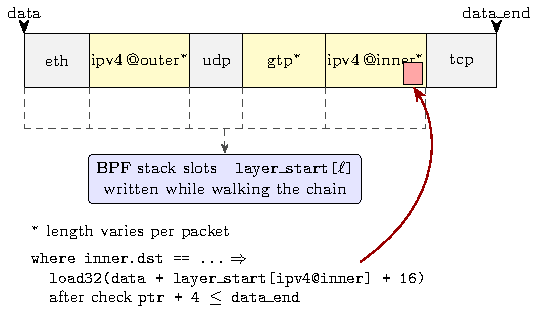
\includegraphics[width=\columnwidth]{figures/fig_layerstart.pdf}
  \caption{Recording each header's start offset into a stack slot, and
  reading \texttt{inner.dst} as a bounds-checked load at layer-start
  $+$ field offset.}
  \label{fig:layerstart}
\end{figure}

Every field access takes the same form: \kunai loads the layer's start
offset, adds the field offset and width, checks the access against
\texttt{data\_end}, loads, and compares. Because type-mismatched
comparisons and a \texttt{proto.field} reference under a repeated
protocol are already rejected at the analysis stage of
\S\ref{sec:overview}, code generation need only emit this bounds-checked
load, even for a chain whose subsequent-header start changes at run time.

\subsection{Lowering Variable-Length Structures to Bounded Bytecode}
\label{sec:bounded}

Because the element count or the length of each element changes per
packet, variable-length structures such as SRv6 segments and TCP
options cannot be walked at a fixed offset. \kunai puts the walk into a
verifier-accepted form by translating it into bytecode with a
compile-time constant bound.

\kunai generates the walk as one of two kinds of bytecode, chosen by
the bound and applied uniformly to chain quantifiers and
\texttt{any()}/\texttt{all()} aux-list walks. A small compile-time bound
within a fixed threshold is unrolled in place. A larger or unbounded one
is lowered to a
\texttt{bpf\_loop} callback with a constant
bound~\cite{bpf_loop_helper}, whose size no longer grows with the
bound. This case covers a parser-machine self-loop, an unbounded chain
quantifier, and a chain or aux-list walk past the threshold.

Algorithm~\ref{alg:walk} gives the shared skeleton. The two lowerings
below fill in its \textsc{stop}, \textsc{stride}, and \textsc{step}
steps, each emitted by its own generator.

\begin{algorithm}[htbp]
  \caption{Bounded walk skeleton; \textsc{stop}, \textsc{stride}, and
  \textsc{step} are filled in per structure.}
  \label{alg:walk}
  \begin{algorithmic}[1]
    \Require $data,\ data\_end,\ base,\ cap$; \textsc{stop}, \textsc{stride}, \textsc{step} per structure
    \State $r \gets \bot$;\ $off \gets base$
    \For{$i \gets 0$ \textbf{to} $cap-1$} \Comment{$cap$: compile-time bound}
      \State \textbf{if} $\textsc{stop}(i, off)$ \textbf{then break} \Comment{count reached, or end/END/malformed}
      \State $ptr \gets data + off$
      \State \textbf{if} $ptr + w > data\_end$ \textbf{then break} \Comment{$w$: bytes read; bounds check}
      \State $r \gets \textsc{step}(ptr)$; \textbf{break if} $r$ decides \Comment{compare, or record option}
      \State $off \gets off + \textsc{stride}(ptr)$ \Comment{constant, or this option's length}
    \EndFor
    \State \Return $r$
  \end{algorithmic}
\end{algorithm}

\kunai fills in this skeleton in two ways, chosen by the structure
rather than the protocol. The compiler classifies each parser loop by
the shape of its states when it loads the protocol definition. A
chain walk over stacked headers such as MPLS needs no loop
classification, since the protocol definition declares the
bottom-of-stack sentinel as a chain-end constant and the quantifier
bound caps the walk. A loop qualifies as a counted aux-list walk
when it extracts elements with \texttt{pkt.extract(stack.next)} under
a \texttt{ParserCounter} seeded from a whole-byte header field and
decremented once per element, so the seed field gives the run-time
count, as \texttt{last\_entry + 1} does for SRv6 in
\figref{fig:p4srv6}. It qualifies as a TLV self-loop when its
\texttt{select} dispatches on a \texttt{lookahead} of the kind byte,
optionally with a byte-count counter as in IPv4 options and Geneve.
The compiler rejects a multi-state parser cycle matching
neither shape at load time rather than compiling it to a wrong walk.

A \emph{counted aux-list walk} handles a list
of fixed-size elements with a run-time count, such as the SRv6 segment
list: \textsc{stop} is $i \geq count$, \textsc{stride} is the constant
element width, and \textsc{step} compares the element field to the
target and decides the walk on a match. For the SRv6 segment filter of
\S\ref{sec:dsl}, \texttt{base = srh\_start + SRH\_FIXED\_SIZE},
\texttt{stride = width = 16}, \texttt{count = last\_entry + 1} (the SRv6
parser's segment-walk seed in \S\ref{sec:p4subset}), and
\texttt{target = fc00::1}.

A \emph{TLV self-loop} handles options that differ in kind and length,
such as TCP options, where a reference like
\texttt{tcp.\allowbreak options.\allowbreak MSS.\allowbreak value} sits
at no fixed offset. Here \textsc{stride} is each option's length,
read at the cursor; \textsc{stop} fires when the cursor reaches the end
of the options, on an END option, on a malformed option (\texttt{len < 2}
or \texttt{cursor + len > options\_end}), or at the iteration bound; and
\textsc{step} dispatches on the option kind and records the position of
the referenced option, which the \texttt{where} clause then reads after
the walk. An option field is loaded only after checking that its option
header stays within the packet window.

In either instantiation, and in either the fixed-unrolling or the
\texttt{bpf\_loop} form, the bound is a compile-time constant and a
bounds check precedes every packet load. The verifier can therefore
confirm both the loop bound and the range of every packet access.

So that the generated bytecode is accepted across kernel versions,
\kunai avoids instructions available only on newer versions. For
byte-order conversion, for example, it uses the \texttt{BPF\_END}
instruction, available on older versions, rather than the
\texttt{BSWAP} instruction introduced in 6.6~\cite{bpf_isa,bpf_cpuv4}.

The building blocks behind these patterns are standard practice in
hand-written eBPF. Programmers routinely place a bounds check against
\texttt{data\_end} before each access and bound every loop by a
constant or by \texttt{bpf\_loop}. \kunai's contribution is not the
techniques but their systematic derivation. The compiler selects and
applies them from the resolved filter structure and protocol
definition, so a filter author writes none of them by hand. Because
\kunai selects the lowering from a structure's shape rather than its
protocol name, GTP-U, SRv6, Geneve, and TCP options need no
per-protocol code in the generator.

\input{sections/05_evaluation}
\section{Limitations}
\label{sec:limitations}

\kunai is a DSL specialized for packet filtering rather than a
general-purpose eBPF language. Stateful filtering, deep packet
inspection, and aggregation are out of scope, and the P4 subset
covers only header layout and parser transitions.

We establish verifier acceptance empirically, without a formal
guarantee~\cite{vishwanathan2022tristate}. Acceptance for an arbitrary
expression on an arbitrary kernel remains future work, and a
\texttt{bpf\_loop} filter has a kernel-version lower bound. The
bytecode is also only as correct as the protocol definition, since p4c
checks P4 syntax rather than agreement with the RFC. Geneve option
TLVs and the tc-stripped outer VLAN tag are not yet filter targets
(\S\ref{sec:eval-accept}).
\section{Conclusion}
\label{sec:conclusion}

We presented \kunai, a packet-filter DSL for the structures
pcap-filter cannot express, such as nested encapsulation, repeated
protocols, and variable-length lists and options. The compiler
resolves filter expressions against protocol definitions written in a
subset of P4, classifies each variable-length structure from the
shape of its parser when the definition is loaded, and lowers it to a
counted walk, a TLV walk, or a sentinel-terminated chain with a
compile-time bound and a bounds check before every packet read.
Because the lowering is derived from structure rather than protocol
names, a new protocol definition extends the filter language without
recompiling the tool. Across six kernels and both attach points, the
generated bytecode was accepted by the verifier, matched and rejected
packets as intended, and stayed within a few percent of pcap-filter
where both languages express a filter. \kunai complements existing
capture tools rather than replacing them. pcap-filter remains a good
fit for filters over fixed header fields, and \kunai takes over where
the target field moves from packet to packet.

\bibliographystyle{ACM-Reference-Format}
\bibliography{refs}

\end{document}
